Le pratiche agili suggeriscono l'utilizzo di \textit{user story} per la descrizione del comportamento del sistema. Una \textit{user story} � una frase, composta utilizzando il linguaggio naturale, che descrive una particolare caratteristica dell'applicazione da implementare.

La struttura della frase da redigere � prefissata e si compone di tre entit� fondamentali: \textit{chi}, \textit{cosa} e \textit{perch�}. Attraverso questi tre concetti � possibile descrivere il comportamento atteso da un attore nel sistema, umano o software, che esegue una determinata azione, al fine di ottenere un risultato.

Ad esempio, per descrivere la \textit{feature} di autenticazione di un utente nel sistema, si potrebbe procedere nel modo seguente:

\begin{quote}
\textit{
\textbf{Come} utente\\
\textbf{Voglio poter} inserire username e password\\
\textbf{Al fine di} accedere al sistema
}
\end{quote}

Come mostra l'esempio, le frasi devono essere concise, in modo da rappresentare una funzionalit� ben definita del sistema.

Le user story sono la prima fase della progettazione e hanno lo scopo, oltre a quello di stilare una lista condivisa di funzionalit� da implementare, di definire un ordine di priorit� e la stima dei tempi di realizzazione delle stesse. Un metodo semplice ed efficace per stimare le user story � riportare il tempo di realizzazione di ognuna a fianco della descrizione.

La \textit{user story} � tipicamente scritta su un biglietto adesivo simile a quello in figura \ref{fig:user-story}, e incollata ad una lavagna che riporta l'insieme dei requisiti del sistema. Un esempio � la \textit{board} in figura \ref{fig:board}.

\begin{figure}[h]
\centering
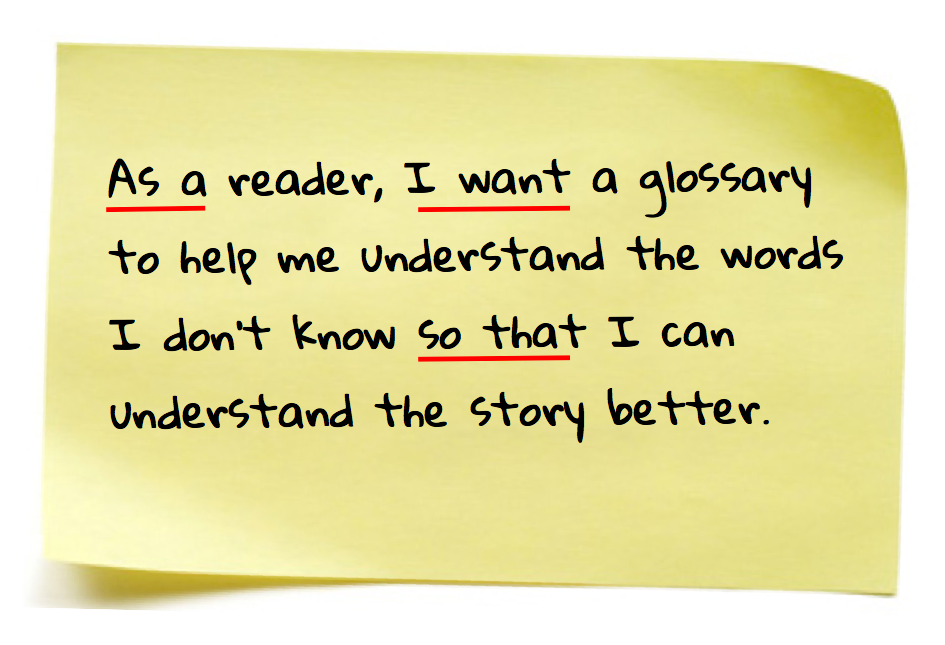
\includegraphics[width=0.7\linewidth]{./img/user-story}
\caption[Un esempio di \textit{user story}]{Un esempio di \textit{user story}}
\label{fig:user-story}
\end{figure}

La creazione delle storie, tipicamente, avviene in collaborazione con il cliente. Durante questo processo l'\textit{owner} lo guida, attraverso domande specifiche, alla stesura e formalizzazione delle funzionalit� necessarie.

Ogni storia rappresenta una feature ben precisa sviluppabile in un periodo che va, tipicamente, da alcuni giorni a un paio di settimane.

L'operazione fisica di scrittura della user story, aiuta il cliente a concretizzare la sua idea di progetto, visualizzandone i dettagli del funzionamento. Questo � molto utile sia per gli sviluppatori, sia per il cliente stesso. Infatti, spesso, i requisiti richiesti non sono dettagliati e specifici a sufficienza. Come ulteriore vantaggio si ha la costruzione di un linguaggio comune, condiviso, tra cliente e sviluppatori che rende agevole la realizzazione dell'intero progetto e dei futuri feedback.

Nel caso in cui le esigenze di progetto cambino, � molto facile, in questo processo, sia sostituire le user story, sia rendersi conto di quale impatto comporti il cambiamento, sull'intero sistema. 

Come sar� descritto nella sezione successiva, l'utilizzo delle user story si lega a quello del TDD, poich� i \textit{test} diverranno la dimostrazione oggettiva dell'effettiva implementazione e garanzia di correttezza di ogni storia.\\

\begin{figure}[h]
\centering
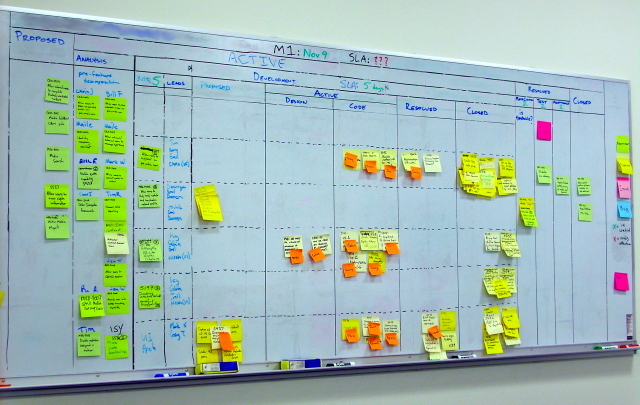
\includegraphics[width=1\linewidth]{./img/board}
\caption[Una lavagna con user story]{Una lavagna con user story}
\label{fig:board}
\end{figure}
